\section{Design}

\newcommand{\POVModel}{\mathcal{M}}

\subsection{Modifying \SfiveN{} in order to simplify the implementation}
In order to simplify the implementation of \SfiveN{}, then instead of an agent $p$ having the entire model $\mathcal{M}$ as described in section \ref{sec:definition-ktfourfiven}, it will have some subgraph of the model $\mathcal{M}$. 
This subgraph will be based on what is able to be seen by $p$. 
So given a model $\mathcal{M} = (W,(R_i)_{i\in \mathcal{A}},L)$ from \SfiveN{}, we are only interested in the worlds $W_{p} \subseteq W$ which are non-contradictory with the current state of the game from $p$'s point-of-view (shortened POV). 
For each $w_p \in W_{p}$, we also keep the worlds which has an equivalence relation to any $w_p$.
For an agent $p$, that has such a model, we denote it $\mathcal{M}_p$ of sub-\SfiveN{}.

\subsubsection{Example of this modification: Three wise men puzzle}\label{sec:motivation}
In order to motivate this modification, I will take the example of the three wise men problem.
There are three wise men, each standing in a row, enumerated 1 through 3. 
Then a king, who has 3 red hats and 2 white hats puts a hat on each of the three wise men in such a way that each person does not know the colour of the hat on their head. 
Then the king asks the first wise man whether he knows the colour of their own hat, where the answer could either be "I don't know" or "I know". 
He then asks the same of the second, then the third.

Let us say that the actual case is RRR i.e. wise man 1, 2 and 3 has a red hat on their head.
In that case wise man 1 will answer: I don't know, the second wise man will answer: I don't know, but the third wise man will answer: I know. How so?



\begin{figure}
	\begin{minipage}[c]{3cm}
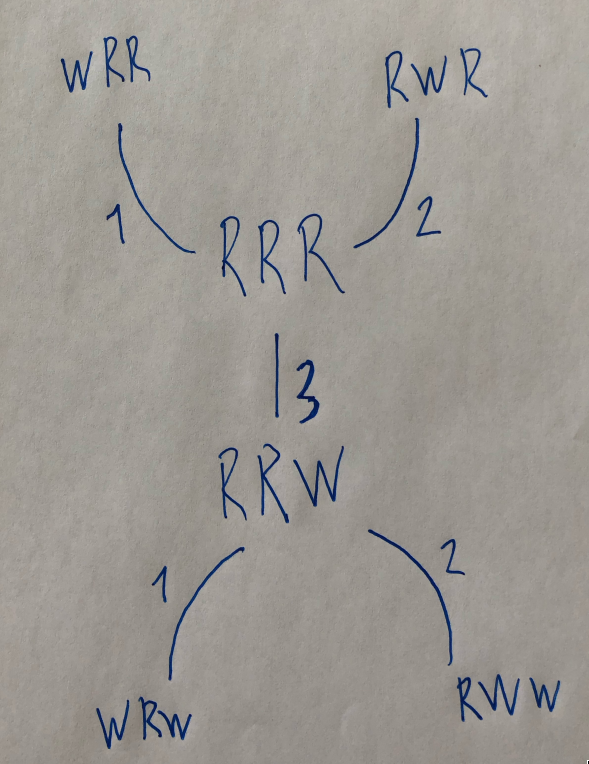
\includegraphics[width=4cm]{images/three_wise_men_round_0.png}
	\caption{The initial model for the third wise man, with no other information than what he can see}

	\label{fig:twm-round-0}
\end{minipage}
\hfill
	\begin{minipage}[c]{3cm}
	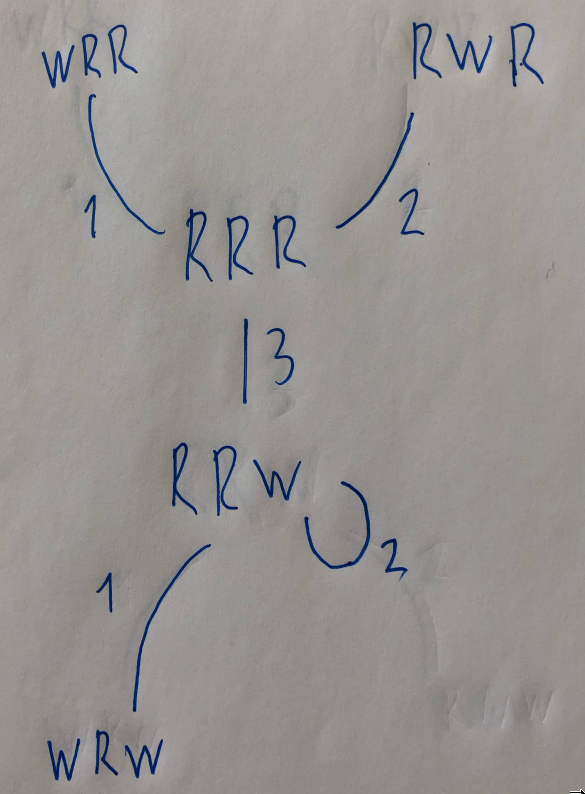
\includegraphics[width=4cm]{images/three_wise_men_round_1.png}
	\caption{The model for the third wise man, after wise man 1 has said "I don't know"}

	\label{fig:twm-round-1}
\end{minipage}
\hfill
	\begin{minipage}[c]{3cm}
	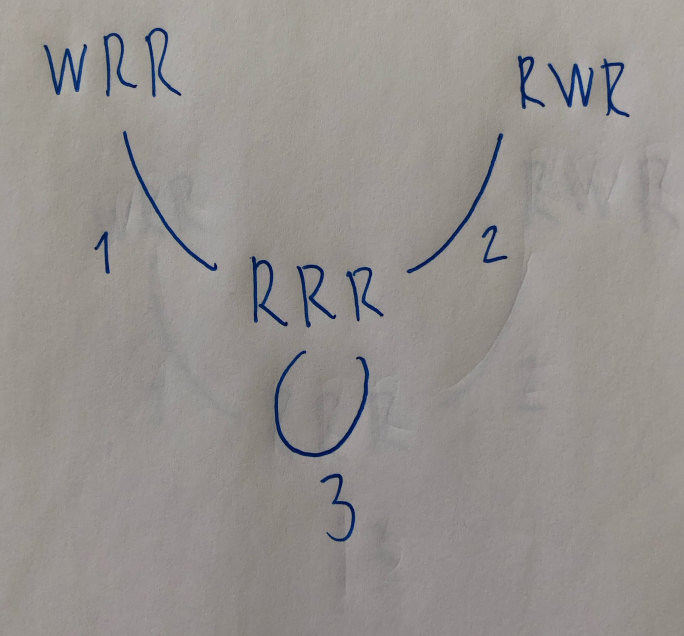
\includegraphics[width=4cm]{images/three_wise_men_round_2.png}
	\caption{The model for the third wise man, after both wise man 1 and 2 have said "I don't know", in succession.}

	\label{fig:twm-round-2}
\end{minipage}
\end{figure}

Figure \ref{fig:twm-round-0} is the $\mathcal{M}_{3}$ model for the initial configuration. 
This means that wise man 3 does not know whether he has a red hat or a white hat. 
And for each of these scenarios he can imagine that 2 cannot know either, and neither can 1. 
I will refer to scenarios that are fixed from a particular player's POV for \emph{fixed scenarios}. 
So here the fixed scenarios are RRR and RRW with respect to wise man 3's model. 
All fixed scenarios implicitly has the equivalence relation $R_3$ in this case, because they are both possible given the information wise man 3 has.

When 1 states "he does not know" then that has to be equivalent to "not RWW is the case". 
This means that three can safely eliminate this state, as something 2 would imagine, given that this was a public announcement. 
This results in the updated model in Figure \ref{fig:twm-round-1}.

After 2 answers "I don't know", wise man 3 can deduce that the case was not RRW, since if it was the case, then 2 would have seen 1:R and 3:W and know that RRW was the only scenario in which this was possible, and hence would answer "I know". 
Which means that the final model that wise man three has is the one on Figure \ref{fig:twm-round-2}, for which the wise man 3 will know with certainty that the only scenario which is possible is RRR.



\subsection{How the subgraph $\mathcal{M}_p$ is generated, given a game-state} \label{sec:description-of-how-modal-logic-is_applied}
Without worrying too much about the combinatorial explosion (more on that later), we can apply the principles described in chapter \ref{sec:motivation} to Hanabi. 

So analogously instead of looking at a world as an assignment of hats, we look at a world as an assignment of hands and contents of the deck, discard pile and colour piles. 
The procedure of generating the model $\mathcal{M}_p$ for an agent $p$ from a set of $n$ agents $\mathcal{A}$ would go like this:

\begin{enumerate}
	\item Generate all fixed scenarios based on the information accessible to $p$. Let's call this set of worlds for $W_p$. 
	\item And make elements in $W_p$ have the relation $R_p$ among each other.
	\item For each $w_p \in W_p$ do
		\begin{enumerate}
			\item For each agent $a \in \mathcal{A}$ do
				\begin{enumerate}
				\item Generate all worlds that $a$ finds possible, given that $w_p$ is the case
				\item Make all elements generated this way have the relation $R_a$ among each other.
				\item Make all elements generated this way, $w_a$, have the relation $R_a(w_a,w_p)$
				\end{enumerate}
		\end{enumerate}
\end{enumerate}

What each agent does not know, is namely their own hand and the contents of the deck. 
If the multiset of cards in the deck was known, then the multiset of cards on their hand would be known and vice versa. 
So we can restrict the problem of generating a world to either have to generate the possible decks, or the their own possible hand. 
I choose to generate their own hand, since it (for the most of the game) is much smaller.
How such a possible hand for some agent $p$ would be generated is to take the multisets of cards
\footnote{because there might be duplicates of the same card}
: The initial full deck $S_{deck}$, the current discard pile $S_{discard}$, the current colour piles $S_{color}$, the other agents' hands $S_{op}$, and find what is left to take from. 
 Then we can see that the set of possible hands $p$ can generate must be taken from the multiset $S_p = S_{deck} \setminus S_{discard} \setminus S_{color} \setminus S_{op}$. 
 The set of hands then is the distinct combinations of size $k$ that we take from the multiset $S_p$.
Here $k$ is 4 or 5 depending on the size of the hand.
Of course this method does not take into account the hands which might conflict with a given set of hints. 
More on this in section \ref{sec:design:removing-worlds-based-on-hints}.


Given the constraints on time and space, it would be nice to have a quite compact representation of each world, furthermore, given that query algorithms will go through most (if not all) of the possible worlds, iterating though the possible worlds should be fast. 
A fast way to iterate through elements is to make sure that each element is small as well as contiguous in order to make use of the CPUs caching system the most, i.e. small elements in a contiguous data structure which guarantees good spatial locality.



\subsection{Formalizing accessing in a model and turning it into an array} \label{sec:model-access}
In order to get good spatial locality I will explain how to take the model of sub-\SfiveN{} and turn it into a multi-dimensional array.

In the section \ref{sec:description-of-how-modal-logic-is_applied} I went through the overall approach of generating the worlds from a specific agent's POV. 
In order to specify how such worlds might be accessed, I extend the solution with some notation. 
Let $\POVModel_p: W \rightarrow P \rightarrow \mathcal{P}(W)$ be the model for the agent $p$'s POV. 
Here the interpretation is that the model takes some fixed scenario $w_p$ of type $W$, and some agent $b$ of type $P$, then we have all the worlds that $p$ cannot rule out that $b$ finds possible, given that $w_p$ is the case.  
The fixed scenarios are strictly from the POV of $p$, which means that all fixed scenarios are all the worlds that $p$ finds possible from the information she has got. 
So all fixed scenarios has an equivalence relation $R_p$. 
The set given by $\POVModel_p(w_p)(b)$ has the equivalence relation $R_b$ among each other, as well as for any $w_b \in \POVModel_p(w_p)(b)$ has the relation $R_b(w_b,w_p)$.
Of course if $b=p$ then we have the unit set, which is simply $\POVModel_p(w_p)(p) = \{w_p\}$.
Which also makes sense in the interpretation "given that we fix the world to $w_p$, then agent $p$ can only imagine that $p$'s only possible world is $w_p$". 

It is clear from the above mapping that this could be encoded using a 3-dimensional array. 
Where $W$ (the first argument) could be interpreted as an enumeration of the fixed scenarios for $p$, and $P$ is an enumeration of the agents, and $\mathcal{P}(W)$ is an array of the possible worlds.


\subsection{Choosing a compact encoding for a world} \label{sec:representing-a-world}
A world is simply a possible state of the entire game, i.e. everything is specified, including the hands you can't see.
A naive approach to representing a world is to take the deck, the discard pile, all of the hands etc. into account.
But this approach is definitely more than necessary, since what is in the discard pile and in the colour pile, as well as most hands, are information easily accessed by the agents themselves, by checking the current state of the game.
Furthermore I choose not to take order into account in any of the hands or piles, because it would lead to too many combinations (a hand of 4 cards has 25 permutations, assuming that all are unique).
What is most interesting to represent is simply then what is uncertain.
So in this case it is a agent's own hand and the current contents of the deck.
Since an agent does not know their own hand, then assuming a hand will give the contents of the deck unambiguously, and vice versa, so it is sufficient to just represent the unknown hand.
So a query $\POVModel_p(w)(b)$, will return the set of hands that $p$ cannot rule out that $b$ finds possible for himself, given that the hand $w$ is the case for $p$.

There are various approaching to representing a hand, I will go through the ones I have devised. 

\begin{enumerate}
\item Represent each card in a sorted order. Called sorted-order representation
\item Enumerate each possible hand. Called Enumeration representation
\item Contingency table inspired multiset. Called table representation.
\end{enumerate}

In each representation I will go through the number of theoretical bits needed per world as well as what the actual number of bits are if we have to make it directly byte-addressable.
The reason I write "theoretical" is due to that most CPU architectures (as well as how Zig compiles code \cite{zigdocspackedstruct}) are byte-addressable.
This means that the smallest addressable space is 1 byte on most modern architectures, even if you want to represent something that uses fewer bits.
The theoretical number of bits can be reached, but it will require some bit manipulation in order to achieve, and comes with the trade-off of more CPU cycles spent extracting the information from a compacted model, rather than accessing the value directly. 


\paragraph{Represent each card in a sorted order}
So firstly we want to look at how small can we get away with representing a card.
A card can be one of 25 different instances (5 suits times 5 values), so a minimal representation could enumerate each card and a world be represented by 5 bits (which can represent from 32 different values).
Then if we have a hand of 4 cards, that means we spent $4 \frac{\text{cards}}{\text{hand}} \cdot 5 \frac{\text{bits}}{\text{cards}} = 20 \frac{\text{bits}}{\text{hand}}$.
And using the same reasoning we use 25 bits for 5 cards.
Then we can predefine some sorted order of the 25 different instances, and just sort a hand in order to get its multiset representation.

If each card has to be byte-addressable then it would have to use 1 byte (8 bits), which would then mean that a hand of 4 cards is 24 bits, and a hand of 5 cards is 40 bits.

Pros: Very simple and compact representation.
No obvious cons.

\paragraph{Enumerate each possible hand}
If you draw 4 cards blindly from an initial deck of 50 cards, there are 18480 distinct combinations (data from Appendix \ref{appendix:python-distinct-combinations}). If it 5 cards drawn it is 99455. 
Depending on the situation, you could enumerate each possible hand.
Then a world need only an integer size large enough to store 18480 or 99455 depending on the case.
This is respectively 15 bits and 17 bits.
So this representation is definitely compact.
Of course some edge-cases exists, for instance in a 5 player game, when the last card has been drawn, then there can exist both 4 and 5 cards representations at the same time, but that would require bits enough to represent $18480+99455 = 117935 < 2^{17}$ so 17 bits should still be sufficient.

Of course if the representation would have to be byte-addressable in an array, then it would have to spent a whole number of bytes, which is respectively 2 bytes (16 bits) or 3 bytes (24 bits).

Of course this enumeration would only create a mapping from an integer to an actual representation, so we would still have to choose a representation that this integer maps to.
Which can be either sorted-order or table representation

Pros: Very compact representation, the enumeration map should only take some constant amount of memory at all times.
Even if we assume the worst case, which is using the table representation and enumerating

Cons: Non-trivial to implement.
A lot of conversion between values i.e. its hard to work on a world directly without looking it up in a map, so when iterating through a list of possible worlds I will have to look up what that world actually is, this I imagine will substantially slow down the algorithm, although I have not tested it.

\paragraph{Contingency table inspired multiset}
I stumpled upon this representation when I was trying to figure out how to generate the possible hands in a fast manner (more on the generation in section \ref{sec:efficient-generation-of-hands}).
Given that instance of a card can at most occur 3 times in a hand (or deck for that matter).
Then an array of 25 elements, each element being able to store 0 through 3, will be a sufficient representation.
This means that each element in the array need only be 2 bits.
So a theoretic use of space is $2 \frac{\text{bits}}{\text{elements}} \cdot 25\text{elements} = 50$ bits. 

If each element has to be byte-addressable then it will have to spent 1 byte per element, in which case $8 \frac{\text{bits}}{\text{elements}} \cdot 25\text{elements} = 200$ bits.
Which is a pretty big increase from the theoretical 50 bits.  

Pros: Very direct multiset representation of the cards, can even be used for the piles and deck. 

Cons: Spends a lot more bits than strictly necessary to represent a world.


\subsubsection{Choosing a representation}
All representations have a convincing set of of trade-offs.
I decided to go with the table representation, since it is very generalizable for other aspects of the game (i.e. can be used to represent decks, piles etc.), as well as easy to work on directly.
Furthermore it is easy generate, see section \ref{sec:efficient-generation-of-hands}.
The other representations should definitely be kept in mind if memory proves to be a problem in practice.


\subsection{Generating hands in an efficient way} \label{sec:efficient-generation-of-hands}
Using the methods described in {\tt math.stackexchange} posts "Efficient algorithm to find all unique combinations of set given duplicates" \cite{HardmathcontigencyTablePost} and \cite{GCabrecursiveGenerationPost}, I was able to design a good generation method for the hands.
The main idea is that we represent the hands we want to generate in a contingency table, where we have some pool to take from.
So a case with hand size of 0 and the pool being the initial deck will be Figure \ref{fig:hand-pool-table} (of course in a practical game, you would know something about the other hands and the discard pile etc. so the pool would be less than the initial deck).
Then the problem is to generate all such contingency tables, such that the sum of the hand is $k$ (usually 4 or 5), and the column sums stay the same, for example see Figure \ref{fig:hand-pool-table-with-hand}.

\begin{figure}
	\centering
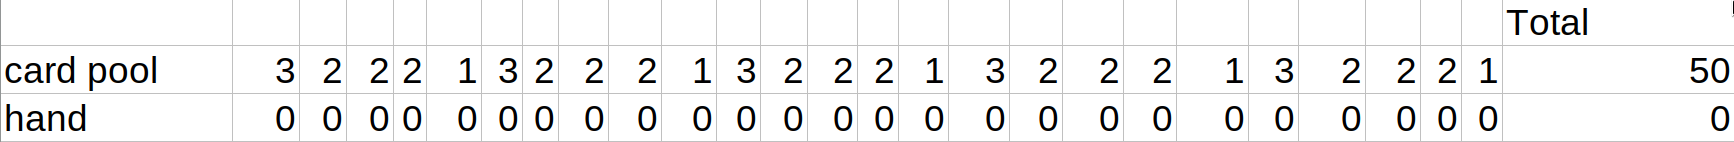
\includegraphics[width=13cm,frame]{images/contigency_table.png}
	\caption{Contingency table with hand size of 0}
	\label{fig:hand-pool-table}
\end{figure}


\begin{figure}
	\centering
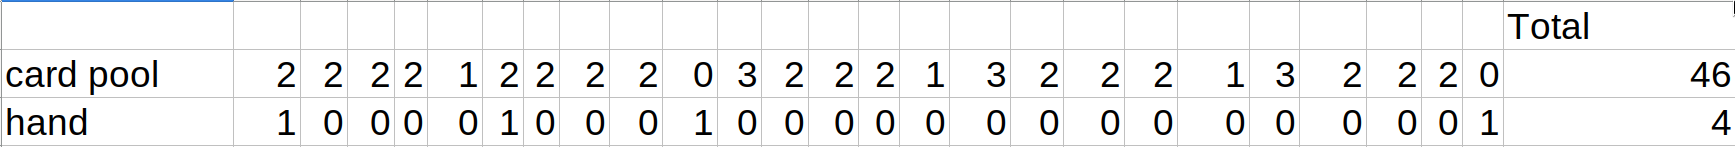
\includegraphics[width=13cm,frame]{images/contigency_table_with_hand.png}
	\caption{Contingency table with hand size of 4}
	\label{fig:hand-pool-table-with-hand}
\end{figure}

Both the card pool and the hand can be represented by using the table representation described in section \ref{sec:representing-a-world}.

The simplest way to describe how the hand is generated, is to view the hand table entries as digits in an integer (or more mathematically specific, a multi-radix integer), with the leftmost digit being the most significant, and then you create the biggest integer with cross-sum $k$, and subsequently construct the number just below that, still with constraint that the cross-sum must be $k$.
So continuing the example with Figure \ref{fig:hand-pool-table}, we can create the "biggest integer" in this way Figure \ref{fig:biggest-integer}.
Then the integer just below that is Figure \ref{fig:next-integer}.
And continuing with 1s until we get Figure \ref{fig:etc-one}.
Then we decrement the most significant digit and get Figure \ref{fig:decrement}.

\begin{figure}
	\centering
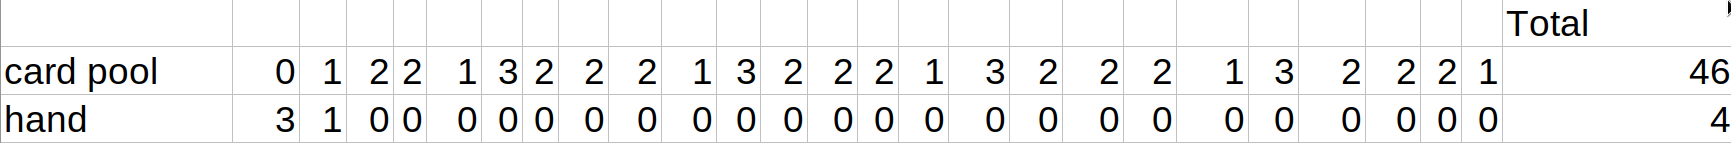
\includegraphics[width=13cm,frame]{images/biggest_integer.png}
	\caption{First generated hand}
	\label{fig:biggest-integer}
\end{figure}

\begin{figure}
	\centering
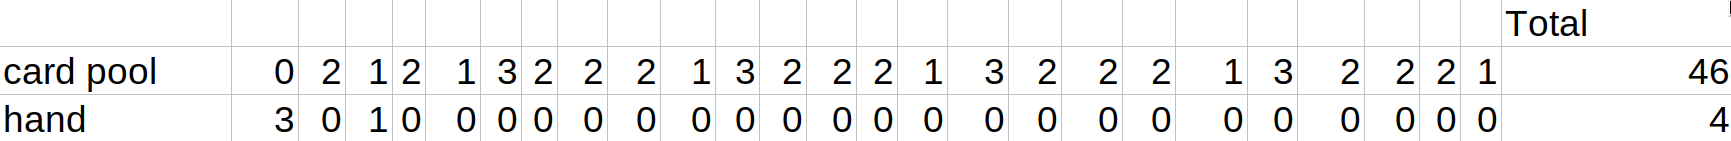
\includegraphics[width=13cm,frame]{images/next-biggest.png}
	\caption{Second generated hand}
	\label{fig:next-integer}
\end{figure}

\begin{figure}
	\centering
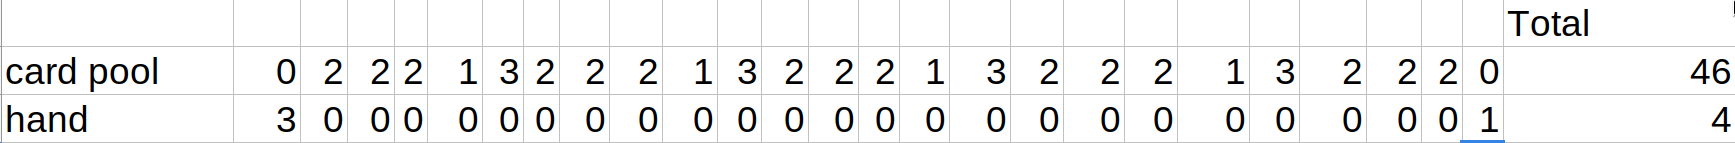
\includegraphics[width=13cm,frame]{images/etc_one.png}
	\caption{The smallest integer containing 3 in the first position}
	\label{fig:etc-one}
\end{figure}


\begin{figure}
	\centering
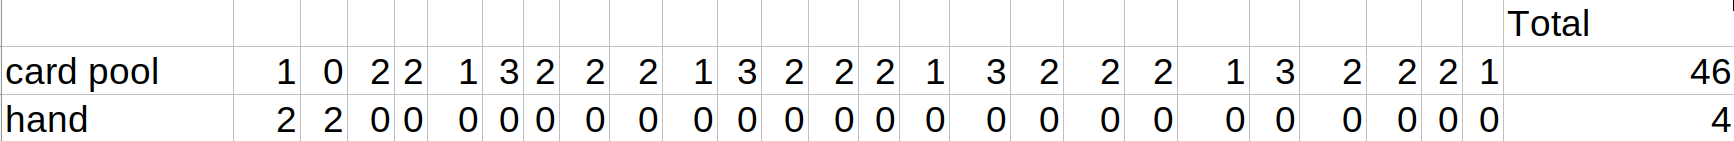
\includegraphics[width=13cm,frame]{images/decrement.png}
	\caption{The biggest integer containing 2 in the first position}
	\label{fig:decrement}
\end{figure}


A more specific algorithmic description is given in section \ref{implementation:sec:generating-distinct-combinations}

\subsection{How should an agent play?} \label{sec:how-should-an-agent-play}

How an agent should play based on its knowledge in sub-\SfiveN{} model is heavily inspired by \cite{CoxEtAl2015}, specifically the information strategy. 
In it they distinguish between \emph{public and private information}.
Where public information is what everybody knows, and everybody knows that everybody knows that etc.
And private information, is what an agent individually knows based on the other agents' hands.

This can be compared to DEL where public information is what the model guarantees is public knowledge, and private information is simply queries that holds true for all possible worlds from that agents POV.

In my solution I will only be querying on the private information. But public information is interesting and is commented on in the Conclusion section.

Given a hand, which is a multiset of known or unknown cards, how does an agent know what card to play based on the private information?
Firstly I will have to decide \emph{when} a card should be played, discarded etc. Here I use the action algorithm from \cite{CoxEtAl2015}, with minor modifications:
\begin{enumerate}
	\item Play the playable card with lowest index.
	\item If there are less than 5 cards in the discard pile, discard the dead card with lowest index.
	\item If there are hint tokens available, give a random hint to a random agent.
	\item Discard the dead card with lowest index.
	\item If a card in the agent’s hand is the same as another card in any agent’s hand, i.e.,it is a duplicate, discard that card.
	\item Discard the dispensable card with lowest index.
	\item Discard index 0.
\end{enumerate}

Here implicitly "playable card", "dispensable card", "dead card", "it is a duplicate", are epistemic queries on the $\POVModel_p$ for the current playing agent $p$'s hand. I denote these types of states a card can be in as \emph{actionable states} for that card.
% So how would an agent go about trying to decide whether a card is playable, discard-able, dead, a duplicate or dispensable? Let's denote each of these states as a card's \emph{actionable states}.

I define the actionable states for a card as follows (also based on \cite{CoxEtAl2015}):
\begin{itemize}
	\item Playable: If it is able to be played in the current game state.
	\item Dead: If the card has already been successfully played and is not needed any more.
	\item Dispensable: If the card could be played at some point (now or in the future), but there is at least one more of the same card left.
	\item Duplicate: There exists a duplicate in another players hand.
\end{itemize}
An agents would eventually have to interpret their hand as a list of cards (where order matters),
due to the fact that they have to play some index from their hand (which they might have full, partial, or no knowledge about).
And it is for this list of cards that the agent has to derive the actionable states for each card, in order to come up with a move.
\todo[inline]{Remember to define player and agent}
But this interpretation of a hand as a list of cards is in contrast to how a world is currently defined: A multiset of cards, where order does not matter.
So we have to define some mapping between an multiset of cards (a world) and a list of cards (the cards on an agent's hand).

To specify how an agent will view it's own hand as a list, we let what is known about a card be denoted by the pair: its suit, and its value. Where it is valid that a suit or value can be "unknown".

As an example: If agent $p$ has the hand ((red,1),(blue,3),(red,2),(yellow,3)), and the current state of the game $p$ only has her red cards hinted, then the list hand $o_{hints}$ would be

\[o_{hints} = ((red,unknown),(unknown,unknown),(red,unknown),(unknown,unknown))\]

In order to create the mapping from a multiset in a world to an list that matches the hand indices, we have to take the hints given to player $p$ into account.

So given an unknown hand for player $p$ specified with the list of hints $o_{hints}$, and the model $\POVModel_p$ we have to decide what possible actionable states is in each card. 

For each fixed scenario for $p$, there is a specific hand for $p$, denoted $h_{specific}$.
Since each hand is stored as a multiset, we have to use the hints $o_{hints}$ to figure out how the set should be mapped to a list.
How this can be done is to make $h_{specific}$ into any list $o_{specific}$ and subsequently take all permutations of $o_{specific}$ and see which ones matches the $h_{hints}$.
If it is possible to find any permutation that is non-contradictory with $o_{hints}$ then we can decide the actionable states for each card given by $h_{specific}$.

Continuing the previous example.
We might have the multiset \[h_{specific} = \{(green,1),(red,5),(green,2),(red,1)\}\]
Turning this into a list we have
\[o_{specific} = ((green,1),(red,5),(green,2),(red,1))\]
we see that there are 4 permutation that matches $o_{hints}$:

\[o_{1} = ((red,5),(green,1),(red,1),(green,2))\]
\[o_{2} = ((red,1),(green,1),(red,5),(green,2))\]
\[o_{3} = ((red,5),(green,2),(red,1),(green,1))\]
\[o_{4} = ((red,1),(green,2),(red,5),(green,1))\]

Then for each permutation we can decide the actionable states of each card, based on the permutation and the current state of the game.
For instance, let us assume that the red colour pile in the current state of the game has a 4 on top.
This means that the card in position 0 can both be playable (if it is a (red,5)), but also be unplayable (i.e. if it is a (red,1)).
Since it is not certain that the card 0 is playable, we cannot perform step 1 in the action algorithm.


\subsection{Removing other players possible worlds based on their hints} \label{sec:design:removing-worlds-based-on-hints}
In section \ref{sec:description-of-how-modal-logic-is_applied} I described how one might generate the possible worlds based on the revealed cards.
Let's say we have two agents $p$ and $b$, and we generate the model $\mathcal{M}_p$.
But there is something important to take into account: if this generation is only based on the cards that are revealed then there will be some possible worlds which conflict with the hints given to $b$, therefore we can also go through all possible worlds for $b$ and remove any that are in conflict with their hints.
This can be done in much the same way as described in section \ref{sec:how-should-an-agent-play}, where we use permutations of a possible world to see if any permutation matches the hints of $b$'s hand.

